\documentclass[a4paper]{report}

\usepackage{amsmath}
\usepackage{amssymb}
\usepackage{amsthm}
\usepackage{tcolorbox} % for colorboxes
\usepackage{minted} % for code highlighting
\usepackage{xcolor} % for own colors
\usepackage[margin=3.8cm]{geometry} % custom page margin
\usepackage{algorithm} % pseudocode
\usepackage{algpseudocode} % pseudocode
\usepackage[german]{babel}
\usepackage{graphicx} % using images

\graphicspath{ {./assets/} } % setting the path for images

% LimeGreen!40
% blue!20
% purple!20
% orange!40
% Emerald!40

\definecolor{dcGrayLight}{gray}{0.95}
\definecolor{dcOrange}{RGB}{255, 128, 0}
\definecolor{dcGreen}{RGB}{117, 225, 102}
\definecolor{dcBlue}{RGB}{99, 203, 255}
\definecolor{dcRed}{RGB}{255,88,88}
\definecolor{dcWhite}{RGB}{255, 255, 255}
\colorlet{dcRedLight}{red!5!white}

\newtcolorbox{definition}[1][]{
    colframe=dcBlue,
    colback = white,
    coltitle = black,
    title = \textbf{Definition}
}

\newtcolorbox{lemma}[1][]{
    colframe=dcGreen,
    colback = white,
    coltitle = black,
    title = \textbf{Lemma}
}

\newtcolorbox{satz}[1][]{
    colframe=dcRed,
    colback = white,
    coltitle = black,
    title = \textbf{#1}
}

\setlength{\parindent}{0in} % remove indentation for paragraphs

\title{Algorithmen und Wahrscheinlichkeiten}
\author{Danny Camenisch (dcamenisch)}

\begin{document}
\maketitle
\tableofcontents
\listofalgorithms


% --------------------------
%   Templates and Examples
% --------------------------

\chapter{Template}
\section{tcolorbox}

\begin{definition}
    Definition...
\end{definition}

\begin{lemma}
    Lemma...
\end{lemma}

\begin{satz}[Satz von Danny]
    Satz...
\end{satz}

\begin{tcolorbox}[colback=dcWhite,colframe=dcOrange,title=\textbf{My Heading}]
    This is a \textbf{tcolorbox}.
\tcblower
    Here, you see the lower part of the box.
\tcbsubtitle{subtitle}
\end{tcolorbox}

\section{minted}

\begin{minted}[frame=lines, framesep=2mm, bgcolor=dcGrayLight, linenos]{java}
    // Hello.java
    import javax.swing.JApplet;
    import java.awt.Graphics;
    
    public class Hello extends JApplet {
        public void paintComponent(Graphics g) {
            g.drawString("Hello, world!", 65, 95);
        }    
    }
\end{minted}

% minted can also import from file like this:
% \inputminted{java}{main.java}


% --------------------------
%   Part 1.
% --------------------------
\part{Graphentheorie}
\chapter{Zusammenhang}

Wir erinnern uns an die Definition eines \textbf{zusammenhängenden} Graphen:

\begin{definition}
    Ein Graph $G = (V,E)$ heisst \textbf{zusammenhängend}, wenn $\forall u,v \in V, u \neq v$ 
    ein Pfad von u nach v in $G$ existiert. \\

    $X$ heisst \textbf{u-v-Seperator}, wenn u und v in verschiedenen Zusammenhangskomponenten von
    $G[V \backslash X]$ liegen.
\end{definition}
\bigskip

Diese Definition besagt zwar ob ein Graph zusammenhängend ist oder nicht, man kann aber nichts darüber sagen,
wie stark ein Graph zusammenhängend ist. Dafür definieren wir sowohl Knoten- als auch Kantenzusammenhang:

\begin{definition}
    Ein Graph $G = (V,E)$ heisst \textbf{k-zusammenhängend}, falls $|V| \geq k + 1$ und $\forall X \subseteq V$
    mit $|X| < k$ gilt: $G[V \backslash X]$ ist zusammenhängend. \\

    Ein Graph $G = (V,E)$ heisst \textbf{k-kanten-zusammenhängend}, falls $\forall X \subseteq E$
    mit $|X| < k$ gilt: $(V, E \backslash X)$ ist zusammenhängend.
\end{definition}
\bigskip

Ein Graph der 3-zusammenhängend ist, besitzt keine Seperator der Grösse 2 und ist dadurch auch 2-zusammenhängend. \\

Anschaulich zu merken: Wie viele Knoten oder Kanten muss man mindestens entfernen, bis der Graph nicht mehr
zusammenhängend ist.

\begin{lemma}
    Knoten-Zusammenhang $\leq$ Kanten-Zusammenhang $\leq$ minimaler Knotengrad
\end{lemma}
\bigskip

Ein (teils schwer zu beweisender) Satz erlaubt uns, eine äquivalente Definition von Zusammenhang
verwenden:

\begin{satz}[Satz von Menger]
    Sei $G = (V, E)$ ein Graph. Dann gilt:
    \begin{enumerate}
        \item $G$ ist k-zusammenhängend $\Leftrightarrow \forall u,v \in V, u \neq v$ gibt es mindestens k intern-knotendisjunkte u-v-Pfade.
        \item $G$ ist k-kanten-zusammenhängend $\Leftrightarrow \forall u,v \in V, u \neq v$ gibt es mindestens k intern-kantendisjunkte u-v-Pfade.
    \end{enumerate}
\end{satz}
\bigskip

\chapter{Artikulationsknoten und Brücken}

\begin{definition}
    Sei $G = (V,E)$ ein zusammenhängender Graph. Ein Knoten $v \in V$ heisst \textbf{Artikulationsknoten}
    (eng. cut vertex) genau dann wenn $G[V \backslash \{v\}]$ nicht zusammenhängend ist.
\end{definition}

\begin{definition}
    Sei $G = (V,E)$ ein zusammenhängender Graph. Eine Kante $e \in E$ heisst \textbf{Brücke}
    (eng. cut edge) genau dann wenn $G[E \backslash \{e\}]$ nicht zusammenhängend ist.
\end{definition}

\begin{lemma}
    Sei $G = (V,E)$ ein zusammenhängender Graph. Ist $\{x,y\} \in E$ eine Brücke so gilt für $x$
    (und analog auch für $y$): \\
    $$deg(x) = 1 \text{    oder    } x \text{ ist ein Artikulationsknoten}$$
\end{lemma}
\bigskip

Die Umkehrung ist hier aber nicht immer wahr! \\

Wie können wir nun solche Artikulationsknoten und Brücken finden? Dazu können
wir eine leicht modifizierte Version der bereits bekannten Tiefensuche verwenden. \\

Dazu müssen wir einige Beobachtungen machen. Zuerst, der von uns gewählte Startknoten $s$ der Tiefensuche,
und, für uns noch viel wichtiger, die Wurzel des Tiefensuchbaums $T$. Es wird schnell klar: Wenn $s$ im Tiefensuchbaum
eine Grad von mindestens 2 hat, so ist $s$ ein Artikulationsknoten. \\

Für jeden Knoten $v \neq s$ ist allerdings nicht so offensichtlich, ob $v$ ein Artikulationsknoten ist oder nicht.
Wieder können wir uns den Tiefensuchbaum zunutzen machen: $v$ ist ein Artikulationsknoten genau dann, wenn
$v$ im Baum Children (oder ganze Subtrees) besitzt, welche keine nicht-Baum-Kante zu einem Vorgänger von $v$ besitzen. \\

Um diese Voraussetzung zu überprüfen, definieren wir für unseren Graphen alle Kanten des Tiefensuchbaums als
\textit{Vorwärtskanten}, alle anderen als \textit{Rückwärtskanten}. Zusätzlich richten wir diese Kanten wie im Baum
(für Vorwärtskanten) bzw. vom höheren zum kleineren DFS Wert für Rückwärtskanten. Weiter definieren wir für jeden Knoten
$v \in V$: \\

low[v] $:=$ kleinste DFS-Nummer, die von $v$ aus durch einen Pfad mit beliebig vielen Vorwärtskanten und maximale
einer Rückwärtskante erreicht werden kann. \\

$
    \text{low}[v] = \text{ min} \left(
        \text{dfs}[v], \underset{(v,w) \in E}{\text{  min  }}
        \begin{cases}
            \text{dfs}[w], \text{ falls }(v,w) \text{ Restkante}\\
            \text{low}[w], \text{ falls }(v,w) \text{ Baumkante}
          \end{cases}
    \right)
$ \\
\\

Dann erhalten wir als Bedingung für Artikulationsknoten:

{\small 
\[
\text{v ist Artikulationsknoten} \Leftrightarrow
\begin{array}{l}
    v = s  v \text{ hat in } T \text{ Grad } \geq 2\\
    v \neq s \text{ und } \exists w \in V \text{ mit }\{v,w\} \in E(T) \wedge \text{ LOW[w]} \geq \text{DFS[v]}
\end{array}
\]
}

Wenden wir unser Wissen über Brücken an, so können wir diese im gleichen Zug berechnen: Eine gerichtete Kante 
${v, w}$ des Tiefensuchbaums (nur diese kommen in Frage) ist eine Brücke genau dann wenn low[$w$] $>$ dfs[$v$].
Restkanten sind niemals Brücken.\\

Unser angepasster DFS-Algorithmus sieht dann wie folgt aus, wobei als Input der Graph $G$ 
und der Startknoten $s$ verlangt wird:

\begin{algorithm}
    \caption{DFS(G,s)}
    \begin{algorithmic}[1]
        \State $\forall v \in V : \text{dfs}[v] \leftarrow 0$
        \State num $\leftarrow 0$ \Comment{Anzahl besuchter Knoten}
        \State $T \leftarrow \emptyset$ \Comment{Menge der Kanten im Tiefensuchbaum}
        \State \Call{DFS-VISIT}{G,s}
        \If{\text{s hat in T mindestens Grad 2}}
            \State isArtVert[$s$] $\leftarrow$ TRUE
        \Else
        \State isArtVert[$s$] $\leftarrow$ FALSE
        \EndIf
    \end{algorithmic}
\end{algorithm}
\pagebreak
\begin{algorithm}
    \caption{DFS-VISIT(G,v)}
    \begin{algorithmic}[1]
        \State num $\leftarrow$ num $ + 1$
        \State dfs[$v$] $\leftarrow$ num
        \State low[$v$] $\leftarrow$ dfs[$v$]
        \State isArtVert[$v$] $\leftarrow$ FALSE

        \For{$(v,w) \in E$}
            \If{dfs[$w$] $= 0$}
                \State $T \leftarrow T + (v,w)$
                \State val $\leftarrow$ \Call{DFS-VISIT}{G,w} \Comment{low-Wert des direkten Nachfolgers}
                \If{val $\geq$ dfs[$v$]}
                \State isArtVert[$v$] $\leftarrow$ TRUE
                    \If{val $>$ dfs[$v$]}
                        \State isBridge[$v$][$w$] $\leftarrow$ TRUE
                    \EndIf
                \EndIf
                \State low[$v$] $\leftarrow$ min\{low[$v$], val\}
            \Else \Comment{Also ist dfs[$w$] $\neq 0$}
                \State low[$v$] $\leftarrow$ min\{low[$v$], dfs[$w$]\}
            \EndIf
        \EndFor

        \State \Return low[$v$]
    \end{algorithmic}
\end{algorithm}


\begin{satz}[Satz]
    In einem zusammenhängenden Graphen $G = (V,E)$, der als Adjazenzlist gespeichert ist, lassen sich
    alle Artikulationsknoten und Brücken in Zeit $\mathcal{O}(|E|)$ berechnen.
\end{satz}
\bigskip

\chapter{Block-Graphen}
\section{Blöcke}
\begin{definition}
    Sei $G = (V,E)$. Wir definieren eine Äquivalenzrelation auf $E$ wie folgt:
    $$e \sim f: \Leftrightarrow e = f \text{  oder  } \exists \text{ Kreis durch } e \text{ und } f$$
\end{definition}
\bigskip

Diese Äquivalenzklassen nennen wir auch \textbf{Blöcke}. Eine alternative Definition lautet wiefolgt:

\begin{definition}
    Sei $G = (V,E)$ ein zusammenhängender Graph. Ein \textbf{Block} ist eine maximale Menge von Kanten, so
    dass je zwei dieser Kanten auf einem gemeinsamen Kreis liegen.
\end{definition}
\bigskip

Merke: Ein Block ist ein Subgraph, der 2-zusammenhängend ist.

\begin{lemma}
    Zwei Blöcke schneiden sich - wenn überhaupt - immer in einem Artikulationsknoten.
\end{lemma}
\bigskip

Wir erinnern uns an die Definition von bipartiten Graphen.

\begin{definition}
    Ein Graph ist \textbf{bipartit}, wenn sich die Knotenmenge in zwei disjunkte Mengen
    $A$ und $B$ zerlegen lässt, sodass Kanten von $G$ nur zwischen $A$ und $B$ verlaufen.
    Wir verwenden dafür folgende Notation:
    $$V = A \uplus B$$
\end{definition}
\bigskip


\section{Block-Graphen}
Ein Block-Graph ist nun wiefolgt definitert:

\begin{definition}
    Der Block-Graph von $G$ ist der bipartite Graph $T = (A \uplus B, E_T )$ mit
    \begin{itemize}
        \item $A =$ {Artikulationsknoten von $G$}
        \item $B =$ {Blöcke von $G$}
        \item $\forall a \in A , b \in B: \{a,b\} \in E_T \Leftrightarrow a$ inzident zu einer Kante in $b$
    \end{itemize}
\end{definition}
\bigskip

\begin{figure}[h]
    \centering
    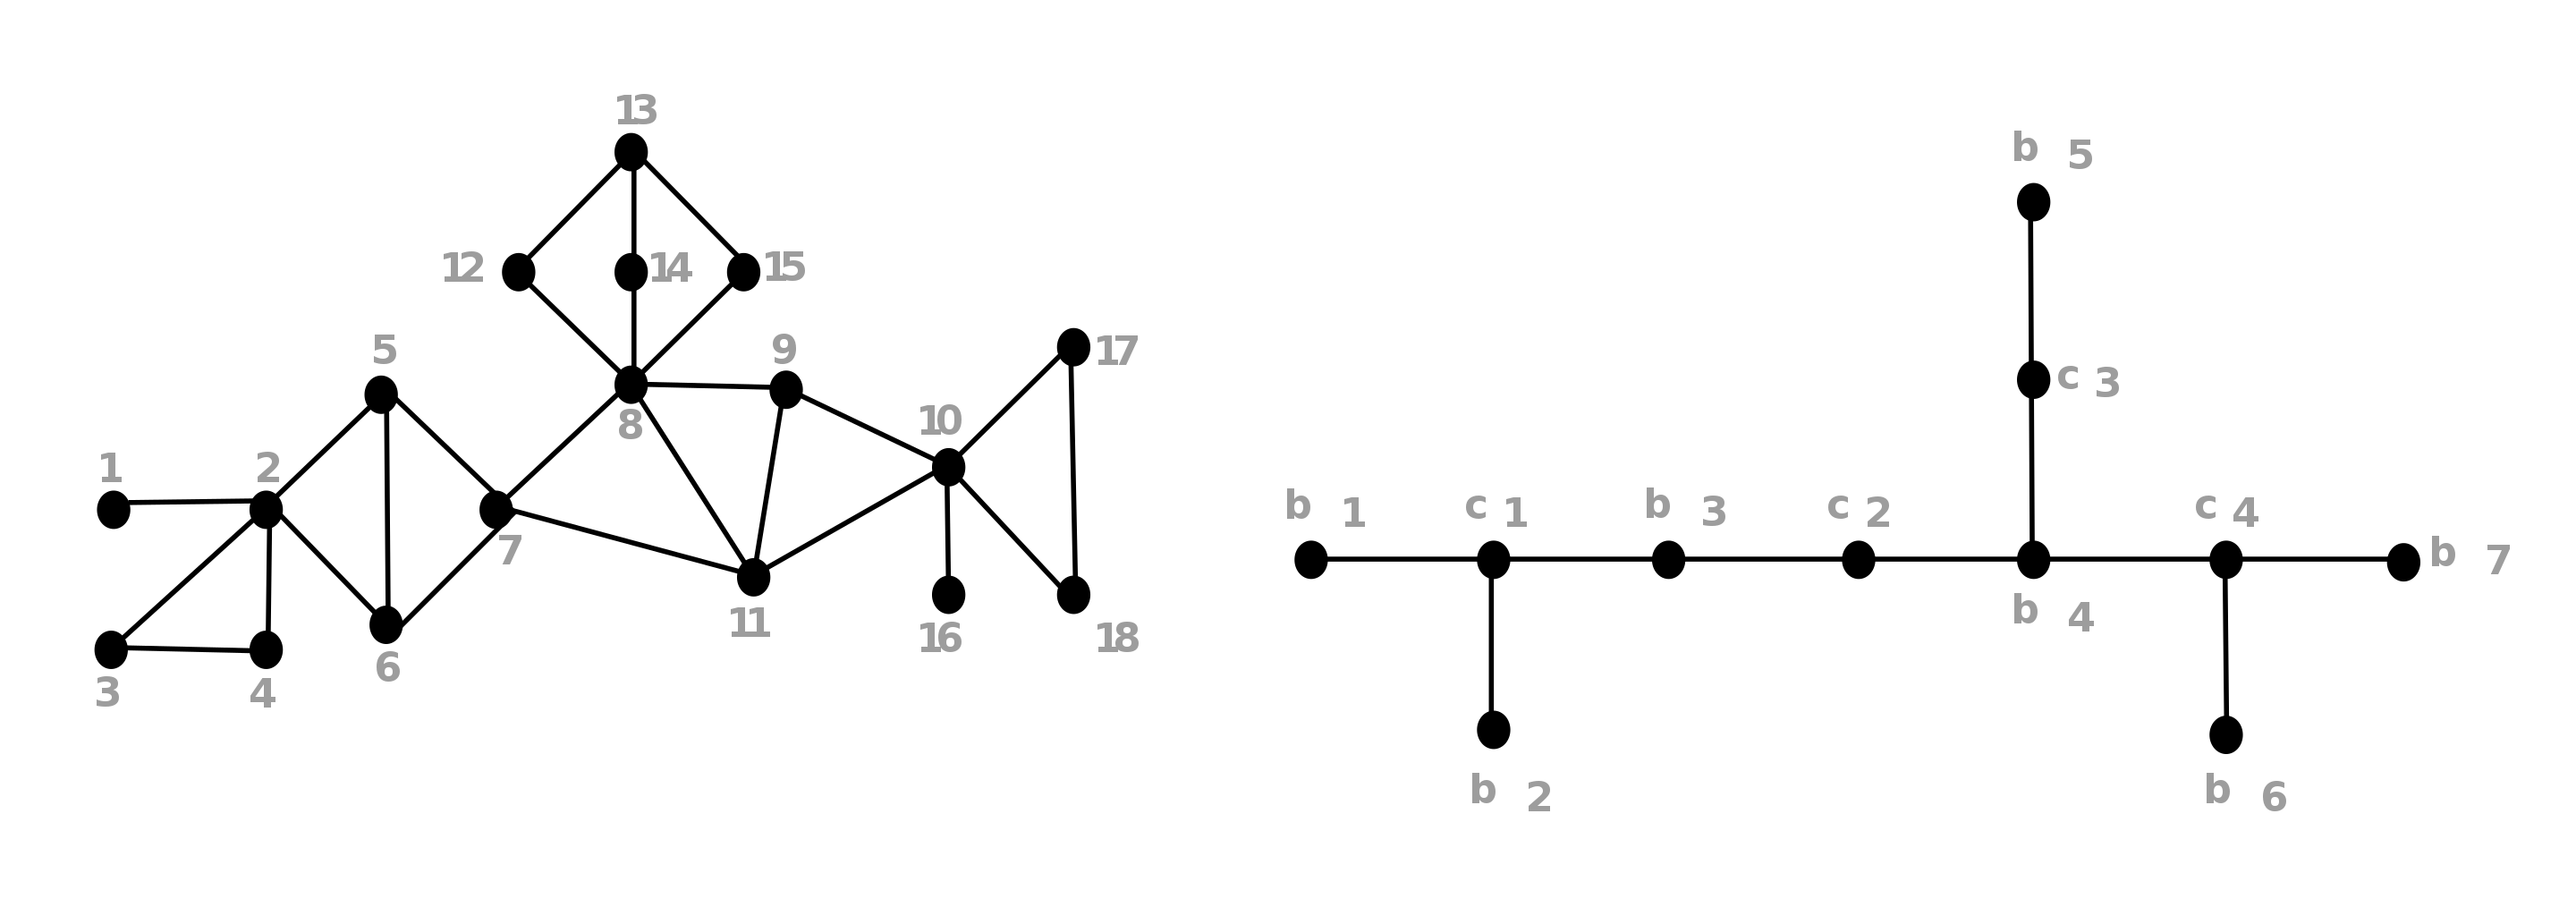
\includegraphics[width=\textwidth]{block_graph.png}
    \caption{Beispiel eines Block-Graphen (links) und der }
\end{figure}


\chapter{Kreise}
\section{Eulertour}
\begin{definition}
    Sei $G = (V,E)$ ein Graph. Eine \textbf{Eulertour} ist ein geschlossener \text{Weg}, der jede Kante genau
    einmal enthält. Enthält ein Graph eine Eulertour, so nennt man ihn \textbf{eulersch}.
\end{definition}
\bigskip

Eine solche Tour lässt sich in $\mathcal{O}(|E|)$ finden - der Algorithmus (''schneller und langsamer Läufer'')
lässt sich ungefähr wie folgt beschreiben:

\begin{algorithm}
    \caption{EULERTOUR(G,s)}
    \begin{algorithmic}[1]
        \State $W \leftarrow$ \Call{RANDOMTOUR}{s} \Comment{''Läufer''}
        \State $v_{slow} \leftarrow $ Startknoten von $W$ \Comment{''Schildkröte''}
        \While{$v_{slow}$ ist nicht der letzte Knoten in $W$} 
            \State $v \leftarrow$ Nachfolger von $v_{slow}$ in $W$
            \If{$\exists (v,w) \in E, w \notin W$} \Comment{Ungenutze Kanten ab $v$}
                \State $W' \leftarrow$ \Call{RANDOMTOUR}{s}
                \State $W \leftarrow W_1 + W' + W_2$
            \EndIf
            \State $v_{slow} \leftarrow $ Nachfolger von $v_{slow}$ in $W$
        \EndWhile
        \Return $W$
    \end{algorithmic}
\end{algorithm}

\begin{algorithm}
    \caption{RANDOMTOUR(s)}
    \begin{algorithmic}[1]
        \State $v \leftarrow s$
        \State $W \leftarrow \{v\}$
        \While{$\exists (v,w) \in E, w \notin W$} \Comment{Ungenutze Kanten ab $v$}
            \State Wähle beliebigen Nachfolger $v_{next}$
            \State Hänge $v_{next}$ an $W$ analog
            \State $e \leftarrow \{v, v_{next}\}$
            \State Lösche $e$ aus $G$
            \State $v \leftarrow v_{next}$
        \EndWhile
        \State \Return $W$
    \end{algorithmic}
\end{algorithm}

Die Laufzeit ist leicht erklärt: Wir betrachten jede Kante genau einmal und "löschen" sie danach.

\begin{satz}[Satz]
    Ein zusammenhängender Graph $G = (V,E)$ enthält eine Eulertour $\Leftrightarrow$ der Grad jedes Knoten
    $v \in V$ ist gerade.
\end{satz}

\section{Hamiltonkreis}
\begin{definition}
    Sei $G = (V,E)$ ein Graph. Ein \textbf{Hamiltonkreis} ist ein Kreis, der alle Knoten von $V$ genau einmal
    durchläuft. Enthält ein Graph einen Hamiltonkreis, so nennt man ihn \textbf{hamiltonisch}.
\end{definition}
\bigskip

Ein klassisches Anwendungsbeispiel ist das Traveling Salesman Problem. Es wird vermutet, dass es keinen 
Algorithmus gibt, der in polynomieller Zeit bestimmt, ob es einen Hamiltonkreis in einem gegebenen Graphen 
gibt. \\

Es gibt aber einige Spezialfälle, für die es deutlich leichter ist, die Existenz eines Hamiltonkreises 
zu bestimmen:

\begin{itemize}
    \item Ein $n \times m$ Gitter enthält einen Hamiltonkreis genau dann wenn $n * m$ gerade ist
    \item Ein d-dimensionaler Hyperwürfel $H_d$ (Knotenmenge: $\{0, 1\}^d$, Kantenmenge: Alle Knotenpaare, welche sich in genau einer Koordinate unterscheiden) enthält einen Hamiltonkreis (auch für Dimensionen $d \geq 4$)
\end{itemize}





Wir bemerken den drastischen Laufzeitunterschied gegenüber der Eulertour: Dort benötigten wir gerade 
einmal $\mathcal{O}(|E|)$ Zeit, um eine solche zu finden, wären das Hamiltonkreisproblem NP-vollständig ist.


\end{document}